\section{\K 三相电路}
\subsection{\K 三相电压}

\Par 交流电产生中我们一般会用到三相发电机,而三相发电机就是单相发电机多加了两个框框而已,这样也能充分利用转子的转动,至于更多框框的五相、七相…由于处理起来比较复杂,就没有用它们.

\Par 我们写出这三个发电机的电源表达式
\begin{equation*}
    \begin{matrix}
        \text{三角函数}&		\text{相量}\\
        \begin{aligned}
        e_1&=\sqrt{2}E\sin \omega t\\
        e_2&=\sqrt{2}E\sin \left( \omega t-120\degree \right)\\
        e_3&=\sqrt{2}E\sin \left( \omega t-240\degree \right)\\
        &=\sqrt{2}E\sin \left( \omega t+120\degree \right)\\
    \end{aligned}&		\begin{aligned}
        \dot{E}_1&=E\angle 0\degree\\
        \dot{E}_2&=E\angle -120\degree\\
        \dot{E}_3&=E\angle +120\degree\\
    \end{aligned}\\
    \end{matrix}
\end{equation*}

用三角函数或相量图像可以表示为
\begin{figure}[htbp]
	\centering
	\begin{minipage}[b]{0.63\textwidth}
        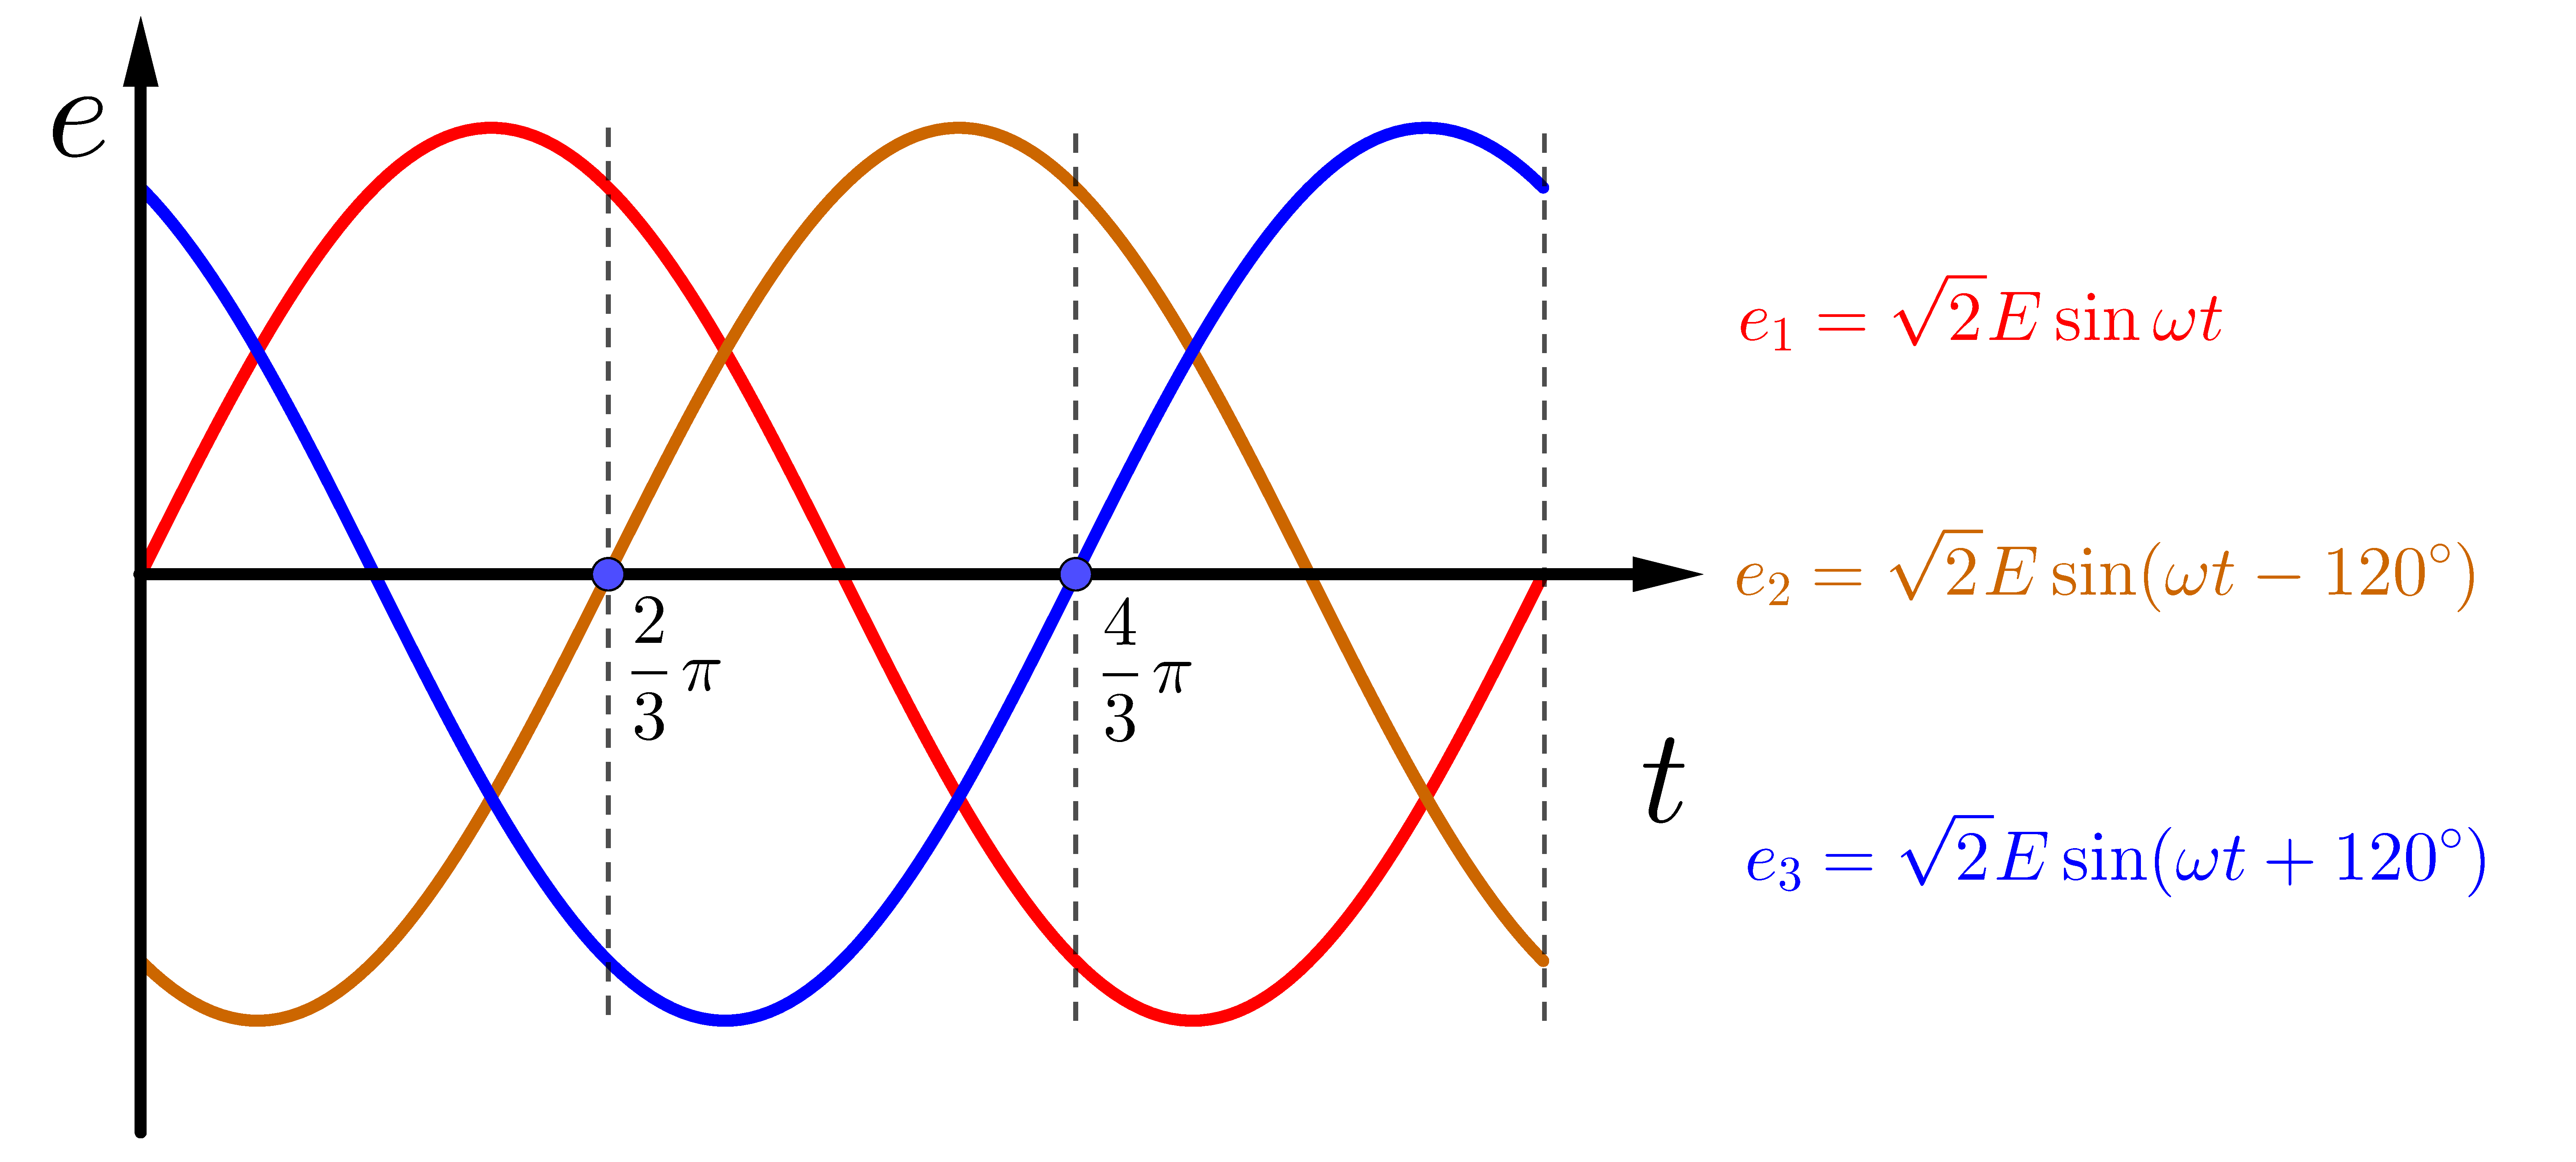
\includegraphics[width=0.85\textwidth]{三相交流电.pdf}
        	\caption{三相交流电}
        	\label{fig:三相交流电}
    \end{minipage}
    \begin{minipage}[b]{0.33\textwidth}
        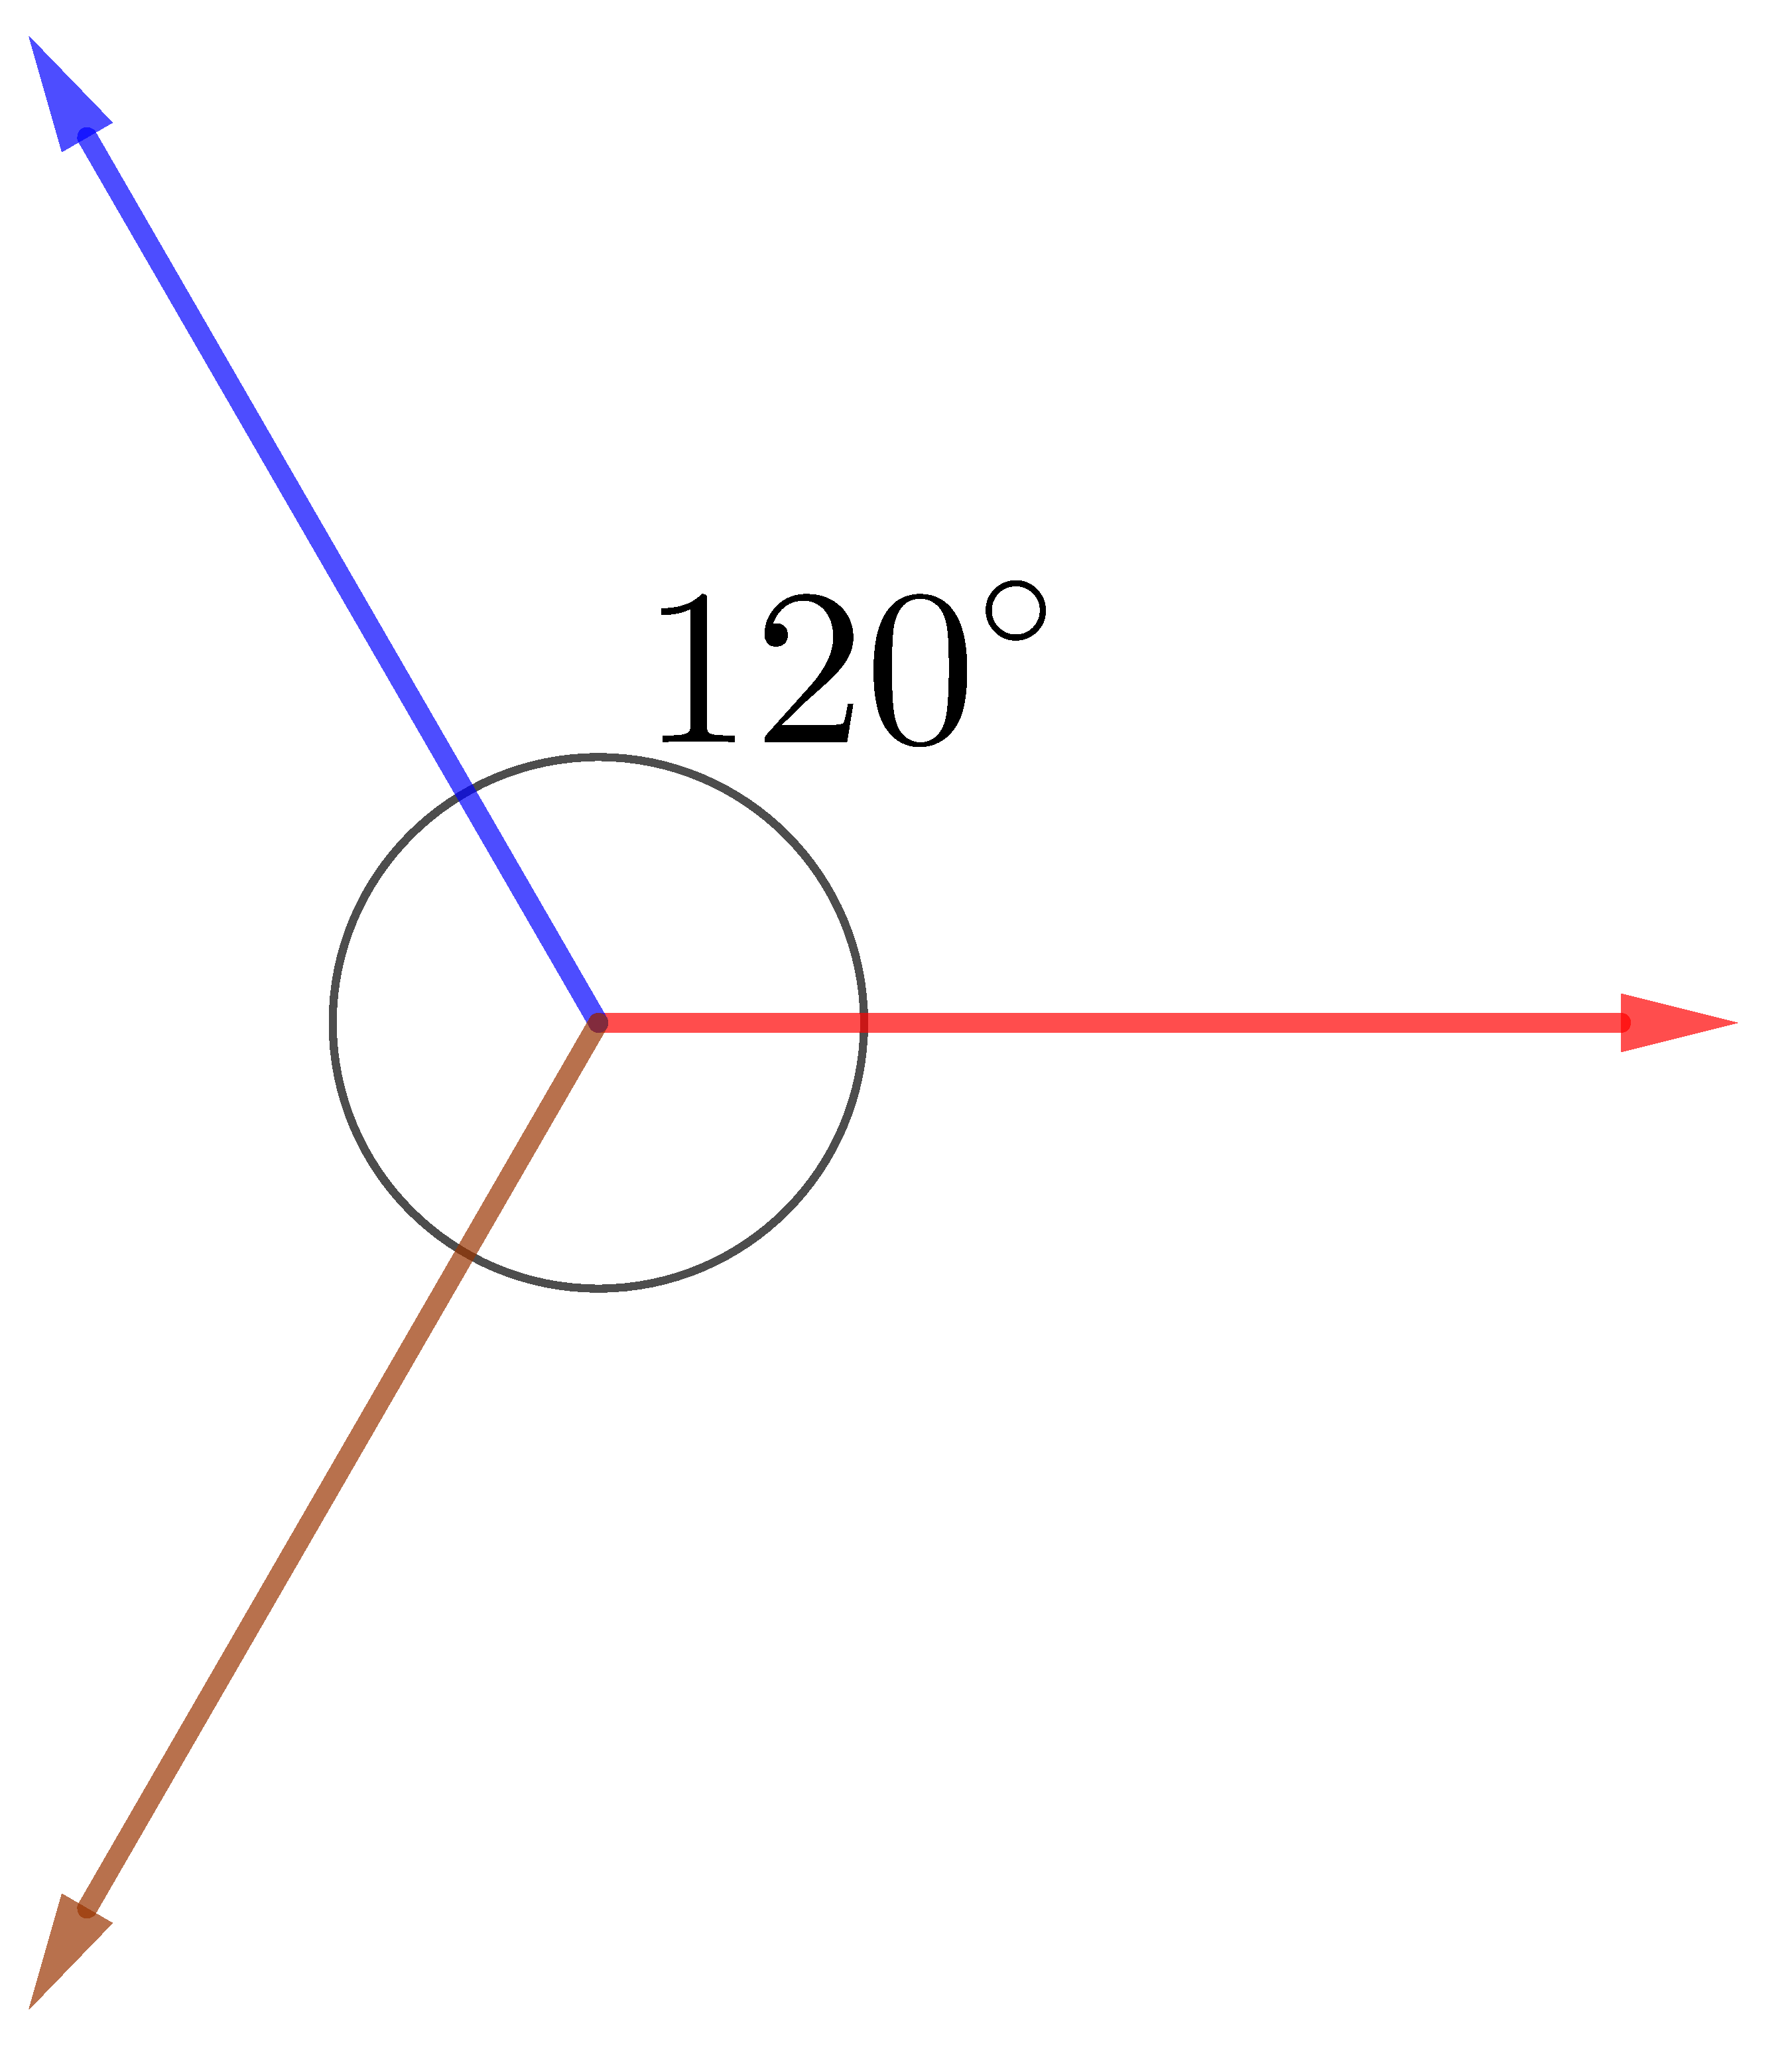
\includegraphics[width=0.85\textwidth]{三相交流电(相量).pdf}
        	\caption{三相交流电(相量)}
        	\label{fig:三相交流电(相量)}
    \end{minipage}
\end{figure}

\Par 可以发现,三个电源仅有相位是不同的,这也是为什么称这种交流电为“三相交流电”的原因.我们规定三个电源到达正向最大的顺序为相序,可见,在图\ref{fig:三相交流电}所示的三相交流电中,它们的相序应该是
\begin{equation*}
    \dot{E}_1\rightarrow \dot{E}_2\rightarrow \dot{E}_3
\end{equation*}

\begin{wrapfigure}[5]{r}{0.35\textwidth}
    \centering
    \includegraphics[width=0.35\textwidth]{三相四线制.png}
    \caption{三相四线制}
    \label{fig:三相四线制}
\end{wrapfigure}
\Par 如图\ref{fig:三相四线制}所示,我们将三个电源的负极接在一起,正极分别连接负载,这样的接线方式被称为\hl{三相四线制}.而这种电源的连接方式被称为\textbf{星形连接法}.负极连接的节点被称为\textbf{中性点},它们共用的负极线被称为\hl{零线},也叫\textbf{中线},它们各自的正极线被称为\hl{火线},也叫\textbf{端线}.同时,我们称上文中提到的电源电压为\hl{相电压},也就是火线与零线之间的电压,记为$U_A$、$U_B$、$U_C$,或者同一记为$U_P$;称相邻两个火线之间的电压为\hl{线电压},记为$U_{AB}$、$U_{BC}$、$U_{CA}$,或者同一记为$U_L$.根据基尔霍夫电压定律,我们可以得到
\begin{equation}
    \left\{ \begin{aligned}
        U_{AB}&=u_A-u_B=\sqrt{6}E\sin \left( \omega t+30\degree \right) =\sqrt{3}E\angle 30\degree\\
        U_{BC}&=u_B-u_C=\sqrt{6}E\sin \left( \omega t-90\degree \right) =\sqrt{3}E\angle -90\degree\\
        U_{CA}&=u_C-u_A=\sqrt{6}E\sin \left( \omega t+150\degree \right) =\sqrt{3}E\angle 150\degree\\
    \end{aligned} \right.  
\end{equation}

可见,线电压的有效值是相电压的$\sqrt{3}$倍,线电压的相位超前于相电压$30\degree$,用三角函数或相量图像可以表示为
\begin{figure}[htbp]
	\centering
	\begin{minipage}[b]{0.63\textwidth}
        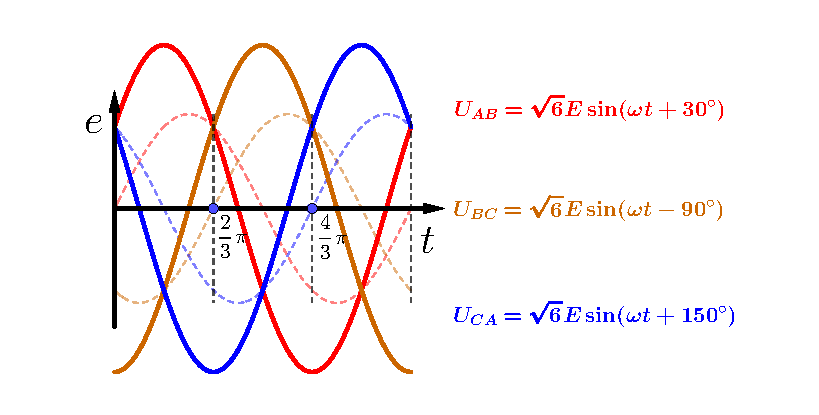
\includegraphics[width=0.85\textwidth]{三相交流线电压.pdf}
        	\caption{三相交流线电压}
        	\label{fig:三相交流线电压}
    \end{minipage}
    \begin{minipage}[b]{0.36\textwidth}
        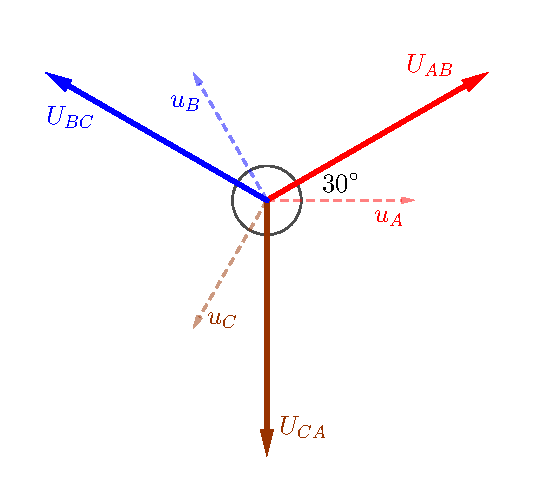
\includegraphics[width=0.85\textwidth]{三相交流线电压(相量).pdf}
        	\caption{三相交流线电压(相量)}
        	\label{fig:三相交流线电压(相量)}
    \end{minipage}
\end{figure}

\subsection{\K 三相负载}

\subsubsection{\K 星形连结}
\Par 对于如图\ref{fig:星形连结负载}所示的星形连结负载,我们先定义:每相负载中的电流$I_P$称为\hl{相电流},每根相线中的电流$I_L$称为\hl{线电流}.在星形连结中,相电流等于线电流,即
\begin{equation}
    I_P=I_L
\end{equation}

\begin{figure}[htbp]
	\centering
	\includegraphics[width=0.65\textwidth]{星形连结负载.png}
	\caption{星形连结负载}
	\label{fig:星形连结负载}
\end{figure}

此时,我们一相一相的计算它的参量,这每一相中的阻抗分别为$Z_1$、$Z_2$和$Z_3$,那么每一相的相电流为
\begin{equation*}
    \left\{ \begin{aligned}
        \dot{I}_1&=\frac{\dot{U}_1}{Z_1}=\frac{U_1\angle 0\degree}{\left| Z_1 \right|\angle \varphi _1}=I_1\angle -\varphi _1\\
        \dot{I}_2&=\frac{\dot{U}_2}{Z_2}=\frac{U_2\angle -120\degree}{\left| Z_2 \right|\angle \varphi _2}=I_2\angle -120\degree-\varphi _2\\
        \dot{I}_3&=\frac{\dot{U}_3}{Z_3}=\frac{U_3\angle 120\degree}{\left| Z_3 \right|\angle \varphi _3}=I_3\angle 120\degree-\varphi _3\\
    \end{aligned} \right. 
\end{equation*}

每相负载中电流的有效值分别为
\begin{equation}
    I_1=\frac{U_1}{\left| Z_1 \right|},I_2=\frac{U_2}{\left| Z_2 \right|},I_3=\frac{U_3}{\left| Z_3 \right|}
\end{equation}
各相负载的电压与电流之间的相位差分别为
\begin{equation}
    \varphi _1=\arctan \frac{X_1}{R_1},\varphi _2=\arctan \frac{X_2}{R_2},\varphi _3=\arctan \frac{X_3}{R_3}
\end{equation}
中性线中的电流可以应用基尔霍夫电流定律得出
\begin{equation}
    \dot{I}_{\mathrm{N}}=\dot{I}_1+\dot{I}_2+\dot{I}_3
\end{equation}
当负载对称时,也就是
\begin{equation}
    Z=Z_1=Z_2=Z_3
\end{equation}
时,因为电压对称,所以负载相电流也是对称的,即
\begin{equation}
    \begin{gathered}
        I_1=I_2=I_3=I_{\mathrm{P}}=\frac{U_{\mathrm{P}}}{|Z|} \\
        \varphi_1=\varphi_2=\varphi_3=\varphi=\arctan \frac{X}{R}
    \end{gathered}
\end{equation}
这时中性线电流等于零,即
\begin{equation}
    \dot{I}_{\mathrm{N}}=\dot{I}_1+\dot{I}_2+\dot{I}_3=0
\end{equation}
此时,地线上没有电流流过,也因此我们不需要地线了,于是便构成了\hl{三相三线电路}.可以发现,只有当负载高度对称时,我们才能使用三相三线电路,否则只能用三相四线电路,此时地线的作用是使电压对称,如果不对称,就会让阻抗大的电分到更多电压,从而烧坏电器.

\Par \hl{短路分析}:当三相四线电路某一相发生短路时,可以发现短路相的短路电流很大,而其他两相的电流保持不变,这时仅需为每一相加上熔断器,就可以在发生短路时保护电器.若是此时将地线断开,那么短路相将没有电流,但是另外两相将会从相电压变为线电压,也就是电压变为原来的$\sqrt{3}$倍,这会烧坏电器,因此不能在地线上装熔断器.

\subsubsection{\K 三角形连结}

\Par 对于如图\ref{fig:三角形连结负载}所示的这样一个三角形连结负载,我们知道相电流不等于线电流,而根据基尔霍夫电流定律,我们可以知道
\begin{equation}
    \left\{ \begin{array}{l}
        \dot{I}_1=\dot{I}_{12}-\dot{I}_{31}\\
        \dot{I}_2=\dot{I}_{23}-\dot{I}_{12}\\
        \dot{I}_3=\dot{I}_{31}-\dot{I}_{23}\\
    \end{array} \right. 
\end{equation}
\begin{figure}[htbp]
	\centering
	\includegraphics[width=0.65\textwidth]{三角形连结负载.png}
	\caption{三角形连结负载}
	\label{fig:三角形连结负载}
\end{figure}

\Par 同时由于没有了地线,这里相电压等于线电压
\begin{equation}
    U_L=U_P=U_{12}=U_{23}=U_{31}=380\mathrm{V}
\end{equation}
各相负载的相电流的有效值分别为
\begin{equation}
    I_{12}=\frac{U_{12}}{\left|Z_{12}\right|}, I_{23}=\frac{U_{23}}{\left|Z_{23}\right|}, I_{31}=\frac{U_{31}}{\left|Z_{31}\right|}I_{12}=\frac{U_{12}}{\left|Z_{12}\right|}, I_{23}=\frac{U_{23}}{\left|Z_{23}\right|}, I_{31}=\frac{U_{31}}{\left|Z_{31}\right|}
\end{equation}
各相负载的电压与电流之间的相位差分别为
\begin{equation}
    \varphi_{12}=\arctan \frac{X_{12}}{R_{12}}, \varphi_{23}=\arctan \frac{X_{23}}{R_{23}}, \varphi_{31}=\arctan \frac{X_{31}}{R_{31}}
\end{equation}
如果负载对称,即
\begin{equation}
    Z=Z_1=Z_2=Z_3
\end{equation}
那么负载的相电流也是对称的,即
\begin{equation}
    I_{12}=I_{23}=I_{31}=I_{\mathrm{P}}=\frac{U_{\mathrm{P}}}{|Z|}\\
    \varphi_{12}=\varphi_{23}=\varphi_{31}=\varphi=\arctan \frac{X}{R}
\end{equation}
此时,线电流有效值等于相电流有效值的$\sqrt{3}$倍,并且线电流相位比相电流滞后$30\degree $,如相量图\ref{fig:相电流与线电流}所示.
\begin{figure}[htbp]
	\centering
	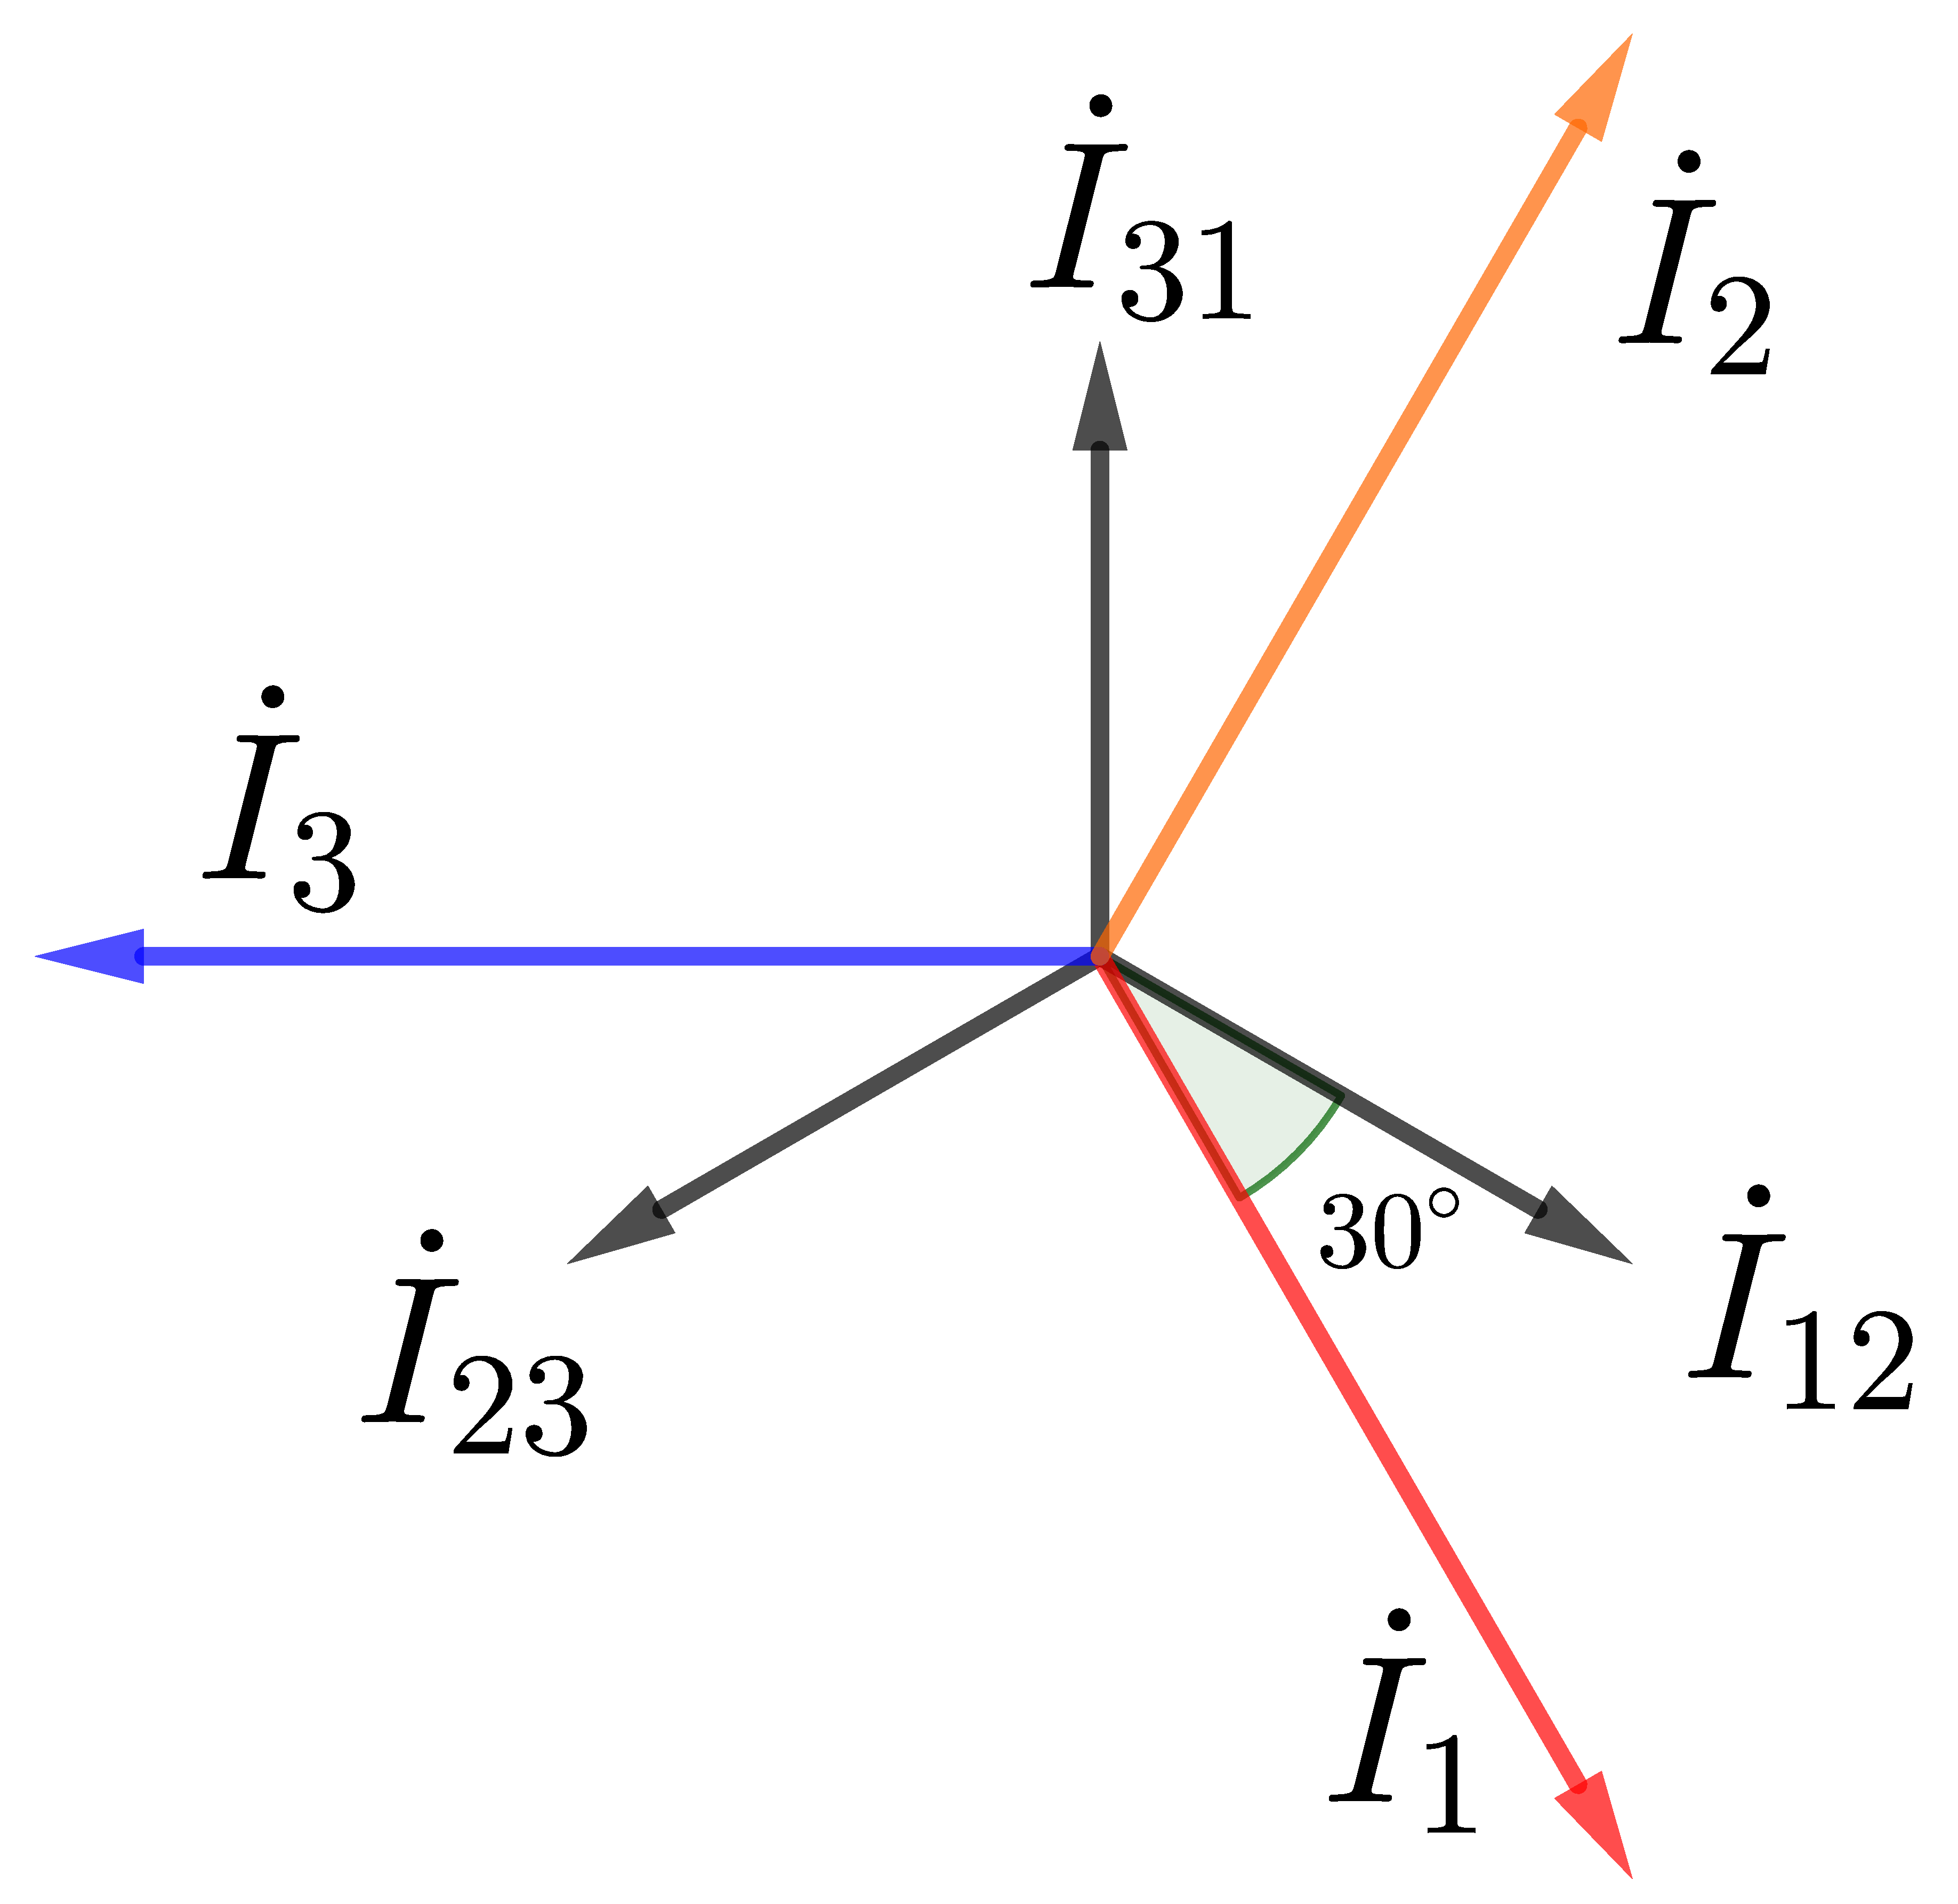
\includegraphics[width=0.45\textwidth]{三角形相线电流.pdf}
	\caption{三角形相线电流}
	\label{fig:相电流与线电流}
\end{figure}

\subsection{\K 三相功率}

\Par 不难知道,三相电路的有功功率等于各项电路的有功功率之和
\begin{equation*}
    P=3P_P=3U_PI_P\cos \varphi 
\end{equation*}
根据星形连结和三角形连结中,线电压和相电压之间的关系以及线电流和相电流之间的关系
\begin{equation}
    \begin{aligned}
        \text{星形连结}&:U_L=\sqrt{3}U_P\,\, ,  I_L=I_P\\
        \text{三角形连结}&:U_L=U_P\,\, ,  I_L=\sqrt{3}I_P\\
    \end{aligned}
\end{equation}
我们不难知道,它们的有功功率用线电压、线电流表示出来都是
\begin{equation}
    P=3U_PI_P\cos \varphi =\sqrt{3}U_LI_L\cos \varphi 
\end{equation}
这里我们之所以要用线电压、线电流表示有功功率,是因为实际测量中线电压、线电流更好测量.同样,我们给出无功功率和视在功率的表达式
\begin{align}
    Q&=3U_PI_P\sin \varphi =\sqrt{3}U_LI_L\sin \varphi\\
    S&=3U_PI_P=\sqrt{3}U_LI_L
\end{align}